\documentclass{book}

%------------------------------------ Packages ------------------------------------
%\usepackage[utf8]{inputenc}
\usepackage{graphicx}
\usepackage{transparent}
\usepackage{import}
\usepackage{color} 
\usepackage{nomencl}
\usepackage{amssymb}
\usepackage{amsmath}
\usepackage[english]{babel}
\usepackage[ddmmyyyy]{datetime}
\usepackage{titlesec}
\usepackage{hyperref}
\usepackage[style=nature,backend=bibtex,maxbibnames=99]{biblatex}
\usepackage{csquotes}
\usepackage[a4paper,lmargin={2.5cm},rmargin={2.5cm},tmargin={2.5cm},bmargin = {2.5cm}]{geometry}
\usepackage{epigraph}
\usepackage[nopostdot,nogroupskip,style=super,nonumberlist,toc,automake,toc]{glossaries}
\usepackage[most]{tcolorbox}
\usepackage[font=small,labelfont=bf]{caption}
\usepackage{titlesec}
\usepackage{tikz}
\usetikzlibrary{trees,fit,shapes}
\usepackage[official]{eurosym}
\usepackage{algorithm}
\usepackage{algpseudocode}
\usepackage{multirow}
\usepackage{booktabs}
\usepackage{array}
\usepackage[flushleft]{threeparttable}
\usepackage{pdfpages}
%------------------------------------ Settings ------------------------------------
% references
\addbibresource{literature.bib} 
\newcommand{\Chapref}[1]{\hyperref[#1]{Chapter~\ref*{#1}}} % capitalize link to chapter

% citation
\newrobustcmd{\twocite}{%
  \AtNextCite{\defcounter{maxnames}{2}\defcounter{minnames}{2}}\fullcite}
  
% \patchcmd{\bibsetup}{\interlinepenalty=5000}{\interlinepenalty=10000}{}{}

% figures
\graphicspath{{figures/}}
\captionsetup[figure]{font=small,justification=raggedright,singlelinecheck=false}
\newcommand{\dummyfig}[1]{
  \centering
  \fbox{
    \begin{minipage}[c][0.33\textheight][c]{0.5\textwidth}
      \centering{#1}
    \end{minipage}
  }
}

% section numbers
\setcounter{tocdepth}{2}
\setcounter{secnumdepth}{2}
\renewcommand{\sectionautorefname}{section}
\renewcommand{\subsectionautorefname}{section}
\renewcommand{\subsubsectionautorefname}{section}
% \titlespacing{\subsubsection}{0pt}{\parskip}{-\parskip}

% color
\hypersetup{colorlinks=true,
linkcolor=black,
filecolor=magenta,
urlcolor=black
}


% line spacing
\renewcommand{\baselinestretch}{1.5}

% footnotes
\renewcommand{\footnotesize}{\fontsize{10}{12}\selectfont}

% numbering
\newcommand{\uproman}[1]{\uppercase\expandafter{\romannumeral#1}}
\newcommand{\lowroman}[1]{\romannumeral#1\relax}

%------------------------------------ Abbreviations -------------------------------
\makeglossaries

%Here we define a set of example acronyms

%%%%%%%%%%%%%%%%%%%%%%%%%% A %%%%%%%%%%%%%%%%%%%%%%%%%%
\newacronym{ai}{AI}{artificial intelligence}

%%%%%%%%%%%%%%%%%%%%%%%%%% B %%%%%%%%%%%%%%%%%%%%%%%%%%
\newacronym{bci}{BCI}{brain computer interface}

%%%%%%%%%%%%%%%%%%%%%%%%%% C %%%%%%%%%%%%%%%%%%%%%%%%%%
\newacronym{crunch}{CRUNCH}{compensation-related utilization of neural circuits hypothesis}
\newacronym{cnn}{CNN}{convolutional neural network}
\newacronym{csp}{CSP}{common spatial patterns}
%%%%%%%%%%%%%%%%%%%%%%%%%% D %%%%%%%%%%%%%%%%%%%%%%%%%%
\newacronym{dmd}{DMD}{dynamic mode decomposition}
\newacronym{dmn}{DMN}{default mode network}

%%%%%%%%%%%%%%%%%%%%%%%%%% E %%%%%%%%%%%%%%%%%%%%%%%%%%
\newacronym{ecog}{ECoG}{electrocorticography}
\newacronym{eeg}{EEG}{electroencephalography}
\newacronym{erm}{ERM}{empirical risk minimization}
\newacronym{erp}{ERP}{event related potential} 
%%%%%%%%%%%%%%%%%%%%%%%%%% F %%%%%%%%%%%%%%%%%%%%%%%%%%
\newacronym{fmri}{fMRI}{functional magnetic resonance imaging}

%%%%%%%%%%%%%%%%%%%%%%%%%% G %%%%%%%%%%%%%%%%%%%%%%%%%%
%%%%%%%%%%%%%%%%%%%%%%%%%% H %%%%%%%%%%%%%%%%%%%%%%%%%%
\newacronym{harold}{HAROLD}{hemispheric asymmetry reduction in older adults}
%%%%%%%%%%%%%%%%%%%%%%%%%% I %%%%%%%%%%%%%%%%%%%%%%%%%%
\newacronym{ica}{ICA}{independent component analysis}
%%%%%%%%%%%%%%%%%%%%%%%%%% J %%%%%%%%%%%%%%%%%%%%%%%%%%
%%%%%%%%%%%%%%%%%%%%%%%%%% K %%%%%%%%%%%%%%%%%%%%%%%%%%
%%%%%%%%%%%%%%%%%%%%%%%%%% L %%%%%%%%%%%%%%%%%%%%%%%%%%
\newacronym{lda}{LDA}{linear discriminant analysis}
%%%%%%%%%%%%%%%%%%%%%%%%%% M %%%%%%%%%%%%%%%%%%%%%%%%%%
\newacronym{mvpa}{MVPA}{multivariate pattern analysis}
\newacronym{mle}{MLE}{maximum likelihood estimation}
\newacronym{mri}{MRI}{magnet resonance imaging}
%%%%%%%%%%%%%%%%%%%%%%%%%% N %%%%%%%%%%%%%%%%%%%%%%%%%%
%%%%%%%%%%%%%%%%%%%%%%%%%% O %%%%%%%%%%%%%%%%%%%%%%%%%%
%%%%%%%%%%%%%%%%%%%%%%%%%% P %%%%%%%%%%%%%%%%%%%%%%%%%%
\newacronym{pasa}{PASA}{posterior–anterior shift in aging}
\newacronym{pca}{PCA}{principal component analysis}
\newacronym{pet}{PET}{positron emission tomography}
%%%%%%%%%%%%%%%%%%%%%%%%%% Q %%%%%%%%%%%%%%%%%%%%%%%%%%
%%%%%%%%%%%%%%%%%%%%%%%%%% R %%%%%%%%%%%%%%%%%%%%%%%%%%
\newacronym{rf}{RF}{random forest}
%%%%%%%%%%%%%%%%%%%%%%%%%% S %%%%%%%%%%%%%%%%%%%%%%%%%%
\newacronym{stac}{STAC}{scaffolding theory of cognitive aging}
\newacronym{svm}{SVM}{support vector machine}
%%%%%%%%%%%%%%%%%%%%%%%%%% T %%%%%%%%%%%%%%%%%%%%%%%%%%
\newacronym{tsne}{t-SNE}{t-distributed stochastic neighbor embedding}
%%%%%%%%%%%%%%%%%%%%%%%%%% U %%%%%%%%%%%%%%%%%%%%%%%%%%
\newacronym{umap}{UMAP}{uniform manifold approximation and projection for dimension reduction}
\newacronym{un}{UN}{United Nations}
%%%%%%%%%%%%%%%%%%%%%%%%%% V %%%%%%%%%%%%%%%%%%%%%%%%%%
%%%%%%%%%%%%%%%%%%%%%%%%%% W %%%%%%%%%%%%%%%%%%%%%%%%%%
\newacronym{who}{WHO}{World Health Organization}

%%%%%%%%%%%%%%%%%%%%%%%%%% X %%%%%%%%%%%%%%%%%%%%%%%%%%
%%%%%%%%%%%%%%%%%%%%%%%%%% Y %%%%%%%%%%%%%%%%%%%%%%%%%%
%%%%%%%%%%%%%%%%%%%%%%%%%% Z %%%%%%%%%%%%%%%%%%%%%%%%%%
%------------------------------------ Document ------------------------------------
\begin{document}
%---------------------------------- Title Page -----------------------------------
\begin{titlepage}
    \begin{center}
        \vspace*{1cm}
        \Huge
        \textbf{WORKING TITLE: Using machine learning aging neuroscience}
                        
        \vspace{1.5cm}
        \LARGE
        By\\
        \vspace{0.5cm}
        \textbf{Christian Johannes Gölz\\}
        \vspace{0.5cm}       
        A thesis presented for the degree of\\
        Doctor rerum naturalium\\
        (Dr. rer. nat)
        \vfill
        \Large
        Paderborn University\\
        Faculty of natural sciences\\
        2022
            
    \end{center}
\end{titlepage}


\pagenumbering{Roman}
\tableofcontents
\chapter*{Acknowledgement}
\addcontentsline{toc}{chapter}{Acknowledgement}
\vspace*{\fill}
\begin{center}
Danke.
\end{center}
\vspace*{\fill}


\chapter*{Abstract}
\setcounter{page}{2}
\addcontentsline{toc}{chapter}{Abstract}
Aim: Apply data science methods to questions in aging Neuroscience\\
Methods: Supervised and unsupervised methods in different settings\\
Results: Novel Data Driven insights\\
Coclusion: ML rocks!


\listoffigures
\addcontentsline{toc}{chapter}{List of Figures}


\listoftables
\addcontentsline{toc}{chapter}{List of Tables}

\printglossary[title={List of Abbreviations}]

\chapter*{Publications and other scientific contributions}
\addcontentsline{toc}{chapter}{Publications and other scientific contributions}
\fullcite{Goelz2021a}\\
\\
\fullcite{Goelz2023}\\
\\
\fullcite{Goelz2021b}\\
\\
\twocite{Gaidai2022}\\
\\
\fullcite{Goelz2018}\\
\\
\fullcite{vieluf2018age}\\
\\
\fullcite{Ströhlein2020}\\
\\
\fullcite{Gowik2023}\\
\\
\fullcite{Strote2020}\\
\\
\fullcite{Strote2020}\\
\\
\fullcite{Niess2022}

\chapter{General Introduction}\label{chap:intro}
\pagenumbering{arabic}

    \section{Motivation}
    \setlength{\epigraphwidth}{0.6\textwidth}
\epigraph{\centering "Humans now live longer than at any time in history. But adding more years to life can be a mixed blessing if it is not accompanied by adding more life to years."} {Dr. Tedros Adhanom Ghebreyesus, WHO Director-General, 2020}

\noindent One of the major societal challenges facing Western societies is the demographic shift towards an older population, which will place enormous demands on society and raise questions about health care, infrastructure, family policy, and employment \cite{WHO_DECADE2020}. To avoid overburdening social structures, one of the main objectives is to promote healthy and independent aging and to improve the quality of life in old age. As part of efforts to promote these goals, the \gls{who} launched the \textit{Decade of Healthy Aging (2021-2030)}, which aims to encourage global action to improve the lives of older adults, their families, and the communities in which they live with the ultimate goal of \textit{adding life to years} \cite{WHO_DECADE2020}.\\
An essential part of promoting healthy aging and enabling participation in society includes the early identification and treatment of pathological conditions, developing and evaluating targeted interventions for prevention and therapy, or designing assistive technologies for older adults. These efforts require a deep understanding of the dynamics of aging in the context of individual trajectories and general patterns. Since many of the mechanisms leading to cognitive and physical decline are related to changes in the brain, it is of great interest to understand and quantify the aging process at this level.\\
Aging is a highly complex phenomenon, and the brain itself, as a nonlinear, dynamic, and multi-layered system, exhibits complex properties in space and time \cite{Betzel2017}. Machine learning offers valuable data-driven methods to unravel this complexity and gain insights by uncovering complex relationships and identifying predictive markers related to the aging process and associated health status.\\
In general, progress in science is more and more characterized by applying methods from \gls{ai}, including machine learning algorithms, which make it possible to systematically analyze large and complex amounts of data \cite{Brunton2019}. This development has led to proclamations of an "\gls{ai} revolution in science" \cite{Appenzeller2017} or promoting science has entered a new area characterized by \textit{data-intensive computing} \cite{Hey2009}. Moreover, these methods serve as the foundations for solving various practical problems, as demonstrated by applications in many socially relevant areas, such as public transport, e.g., autonomous or self-driving vehicles \cite{Leonard2020}, the medical sector, e.g., diagnostic imaging \cite{Liu2020}, or social interaction, e.g., tools for communicative interaction \cite{Adamopoulou2020}, and are thus one of the basic building blocks for assistive technology facilitating the participation of older people with disabilities in society. \Gls{ai} and machine learning as a key technology have become a hope for solving societal challenges, including the shift towards an older population.\\
However, the implementation of machine learning approaches in aging research is still at an early stage compared to the rapid development in the commercial sector, and the most effective applications and integration into the traditional scientific system have yet to be evaluated, despite the potential to better understand the aging brain.\\
This is the starting point of this dissertation which aims to investigate brain aging using machine learning techniques. The focus is on using these methods to better understand the neurophysiological factors contributing to age-related sensory, motor, and cognitive changes. To this end, existing hypotheses about the aging brain will be tested and validated while new hypotheses will be generated. The results inform the development of assistive technologies to facilitate the participation of older adults in society, the early detection of pathological conditions, or the development of targeted interventions to counteract age-related decline.

\section{Outline}
This dissertation is separated into five main chapters. This \hyperref[chap:intro]{chapter} describes the thesis's theoretical framework. In \chapref{theory:aging}, a description of aging at the level of the brain focuses on the most relevant concepts for the context of this work and forms the starting point for introducing the added value of applying machine learning in the context of studying the reorganization of the aging brain. Next, machine learning is introduced in \chapref{theory:ml} to provide the methodological framework. The general terminology and a literature-based overview of the use of machine learning methods in neuroscience and especially in the neuroscientific research on aging will form the basis for the deduction of the research aim and scope of this thesis in the following \chapref{chap:aims_scope}. \chapref{chap:methods} includes a description of the general methodological approaches of this work. In the subsequent \chapref{chap:results}, the main results of the published research articles underlying this thesis will be presented. These include:

\begin{itemize}
\item Research Article \uproman{1}:\\ \hyperref[pub:paperI]{Goelz, C. \textit{et al.} Classification of visuomotor tasks based on electroencephalographic data depends on age-related differences in brain activity patterns. \textit{Neural Networks} \textbf{142}, 363--374 (2021)}
\newpage
\item Research Article \uproman{2}:\\ \hyperref[pub:paperI]{Goelz, C. \textit{et al.} Classification of age groups and task conditions provides additional evidence for differences in electrophysiological correlates of inhibitory control across the lifespan. \textit{Brain Informatics} \textbf{10}, 11 (2023)}
\item Research Article \uproman{3}:\\ \hyperref[pub:paperI]{Goelz, C. \textit{et al.} Electrophysiological signatures of dedifferentiation differ between fit and less fit older adults. \textit{Cognitive Neurodynamics} \textbf{15}, 1--13 (2021)}
\item Research Article \uproman{4}:\\ \hyperref[pub:paperIV]{Gaidai, R., Goelz, C., \textit{et al.} Classification characteristics of fine motor experts based on electroencephalographic and force tracking data. \textit{Brain Research} \textbf{1792}, 148001 (2022)}
\end{itemize}

\noindent The thesis concludes with an overreaching discussion in which the results are evaluated in the light of the current scientific discourse highlighting practical implications and future research topics (\chapref{chap:discussion}). 

    \label{motivation}

    \section{Aging}
    \label{theory:aging}
    Biologically aging can be broadly characterized as "the time-dependent functional decline that affects most living organisms" \cite{López-Otín2013}. It can be observed in the reorganization of multiple interacting physiological systems operating at different spatial and temporal scales \cite{Mooney2016}. The underlying patterns of reorganization within and between these systems are highly individual, as they are subject to internal (e.g., genetic, cellular, molecular) as well as external (e.g., environmental, and lifestyle) influences \cite{Smith2020, Mooney2016, Cohen2022}. At the same time, however, overarching, generalizable patterns can be identified \cite{Salthouse2019}. The most recognizable consequences of aging are alterations in cognitive, sensory, and motor abilities that challenge the daily lives of older adults \cite{Li2002}. However, not all abilities are equally affected by declines and the alterations are highly individual. While sensory, motor abilities and cognitive abilities, such as memory and processing speed, are described as generally declining, abilities in the context of acquired knowledge, such as verbal abilities, tend to be stable or even improve with age \cite{Park2009}. Understanding brain reorganization is of particular interest because of its interrelation with behavioral alterations.

\subsection{Age-related reorganization of the brain}
\label{theory:aging:brain}
Reorganization in the structure of the brain include, among others, atrophy of the gray and white matter as well as enlargement of cerebral ventricles \cite{Fjell2010}. The efficiency of neuromodulation declines mainly driven by the loss of dopaminergic receptors indicative of a reorganization of neurotransmitter systems \cite{Li2001}. Besides this, the study of the functional properties of the brain and their relationship to behavioural changes is of great interest. In neuroimaging studies, both under-activation and over-activation of brain areas have been reported in older adults compared to younger adults during performance in various tasks with sensory, cognitive as well as motor demands \cite{Reuter-Lorenz2010, Sala-Llonch2015}. In terms of activation dynamics, brain activity in response to a stimulus is often slower or delayed. Moreover, the frequency distribution of neural oscillatory activity changes with respect to a slowing of the main rhythms and altered temporal dynamics which is interpreted as changes in neural communication \cite{Courtney2021}.\\ 
By emphasising neural communication and information flow, rather than viewing the brain as functionally separate, it can be conceptualised as a complex system whose functional units, i.e. neurons, areas and subsystems, are interconnected both structurally and functionally \cite{Friston2011,Deery2023}. In this concept, functional connectivity reflects coherent patterns of activation within and between these units. Several distinct but interconnected functional networks were identified. The dynamic interplay between and within these networks is characterized by segregation and integration at different levels, characterizing the flow of information in the brain \cite{Sporns2013}. Older adults information flow tend be less efficient and is characterized by lower within network connectivity and higher between network connectivity associated with a less segregated, less modular and more integrated brain network organization \cite{Sala-Llonch2015,Deery2023, Betzel2014}. However, studies on sensorimotor and visual networks seem to be very heterogeneous, which could indicate very individual reorganization patterns \cite{Deery2023}.

\subsubsection{Dedifferentiation}
\label{theory:aging:dedif}
The functional reorganization patterns described in the previous section have been be attributed to dedifferentiation \cite{Grady2012}. Dedifferentiation refers to the loss of neural specialization or reduced distinctiveness of neural responses resulting in a diffuse, non specific recruitment of brain resources \cite{Koen2019}. Historically, the term originates from behavioral research in which an increased correlation of performance between sensory, cognitive and sensorimotor domains was reported in older adults \cite{Baltes1997,Li2002}. In order to explain this behavioral dedifferentiation Li and colleagues \cite{Li2001, Li2002} provided a computational model. According to this model, deficient neurotransmitter modulation observed in older adults may affect the responsiveness of cortical neurons, leading to higher levels of neuronal noise and ultimately to less differentiated, more diffuse neuronal activation patterns in response to different stimuli \cite{Li2001,Li2002} (see Figure \ref{fig:dedifferentiation} for an overview on the computational model). In several computational simulations, the authors demonstrated that the proposed model can explain not only behavioral co-variation, but also several other phenomena, such as the decrease in average behavioural performance or the increase in behavioral intra- and inter-person variability \cite{Li2000,Li2002}. In addition, the proposition of a less distinctive, less specific neuronal activation in response to stimuli could be confirmed in neuroimaging studies showing that the neural responses to various visual, cognitive and motor stimuli are less specific in older compared to young adults \cite{Tucker2019, Koen2019,Carb2011}. 

\begin{figure}[h]
\def\svgwidth{\columnwidth}
\input{figures/dedifferentiation.pdf_tex}
\caption[The computational model proposed by Li and colleagues \cite{Li2000,Li2002}]{The computational model proposed by Li and colleagues \cite{Li2000,Li2002}. The authors used a feedforward backpropagation neural network model with logistic activation function $f(z)$ and simulated altered neuromodulation by varying the gain parameter $g$ in $f(z)$ of each neuron (A). Deficient neuromodulation and responsiveness due to aging is simulated by lower $g$ values resulting in a dampened activation of a neuron (B). Simulations showed that the activation pattern of simulated neurons differs less for different stimuli, i.e. the hidden layer of the network shows a less distinctive representation of the stimulus (C). The activation of a single neurons is more variable for multiple stimulations with the same stimulus (D).}
\label{fig:dedifferentiation}
\end{figure}

\noindent Recently the reorganization of functional networks as described above, i.e. less segmented and modular, and less specialized organization in older adults was framed in terms of dedifferentiation \cite{Deery2023, Koen2019, Sala-Llonch2015}. \citeauthor{Fornito2015} \cite{Fornito2015} describe dedifferentiation as a fundamental maladaptive mechanism of brain networks that requires compensation. This is consistent with the argument that dedifferentiation and compensation are complementary mechanisms \cite{Reuter-Lorenz2010}. However, dedifferentiation could also itself represent a compensatory response, in that the brain attempts to maintain function in the face of deterioration \cite{Stern2009}. By definition compensation refers to the ability to recruit additional brain resources to compensate for decline and functional loss in order to maintain cognitive or behavioural functioning \cite{Reuter-Lorenz2010, Grady2012}. Here, the \gls{crunch} hypothesizes that compensatory activity changes as a function of task demands. Moreover, compensation often occurs in a specific pattern of under-activation of posterior areas and prefrontal over-activation, known as \gls{pasa} \cite{Davis2007}. Another often reported pattern is the more bilateral recruitment and loss of hemispheric specialization, known as \gls{harold} \cite{Cabeza2002}.

\subsubsection{Reserve}
\label{theory:aging:reserve}
It is important to note that age-related alterations of the brain and behavior are highly individual and dynamic \cite{Smith2020,Koen2019,Douw2014}. In this context, the concept of reserve was defined as the accumulated capacity of neural resources over the lifespan that can withstand decline or pathology \cite{Cabeza2018, Stern2009}. Although the concept was originally based on observations that the degree of pathological changes in the brain do not necessarily mean clinical manifestation, it has also been applied to explain individuality of non-pathological aging \cite{Esiri2001,Cabeza2018,Stern2009}.\\
Reserve can be both anatomically quantifiable, which is referred to as brain reserve, and more functional in nature, which is referred to as cognitive reserve \cite{Stern2009}. At the functional level, compensatory activation as well as more efficient utilisation (less activation of neural resources), increased capacity (increased availability of neural resources) were described as key mechanisms of cognitive reserve \cite{Stern2004,Stern2009}. Brain and cognitive reserve influence each other and \citeauthor{Cabeza2018} \cite{Cabeza2018} argue against a strict separation of brain reserve and cognitive reserve.\\
One aspect that explicitly determines the definition of reserve is the lifelong ability of the brain to adapt its structure and function to internal and external requirements. It is known from the animal model that environments rich in cognitive, social, as well as sensory and motor stimuli, contribute to positive plastic changes \cite{Fabel2009}. As a result, reserve is influenced by an interplay between genetic and environmental factors including lifestyle factors \cite{Cabeza2018}. Important factors for increasing reserve have been identified in education, occupation as well as physical activity, with cognitive training, physical fitness, and professional expertise having a considerable impact on the brain's functional organization \cite{vieluf2018age,VOSS2016113,Soldan2021}.\\
This is further supported by other complementary concepts such as the maintenance or the \gls{stac} models. The concept of maintenance emphasizes the ability to repair. \Gls{stac} postulates that lifelong positive and negative plasticity define a framework that enables compensation and shapes the individual trajectory of aging \cite{Reuter-Lorenz2014}. 

\subsection{Studying brain aging by electroencephalography}
The complex interplay of the aforementioned factors leading to the dynamics of age-related reorganization of the brain is highly complex. Understanding these dynamics in terms of individual trajectories and overarching patterns is a prerequisite to differentiate healthy from pathological changes and to develop and verify treatments as well as targeted interventions. This requires uncomplicated, easy-to-use, and cost-effective methods and novel analyses to quantify changes in brain organization. Several noninvasive methods are available to study the brains' structure and function. \Gls{mri} is the most widely used method in science to image the structure or, using \gls{fmri}, the function of the brain, which is the dominant method in the study of the functional reorganization described in the previous section \cite{Reuter-Lorenz2010}. However, this method is very costly and requires expertise that is not widely available. As a result, its use in the public health system is mostly limited to cases with a clear indication, so that early detection of unfavourable aging trajectories is rather difficult. In addition, limited availability substantially restricts the development of preventive and rehabilitative interventions and therapies and excludes areas and sites with low levels of equipment and expertise. Here, \gls{eeg} could represent a real added value, since it is characterized by a simple use, mobility, and relative cost effectiveness. Although it has a lower spatial resolution than \gls{mri} based methods, \gls{eeg} measures neuronal activity directly with high temporal resolution which allows for the detection of age-related changes in the temporal dynamics of brain activity and networks, which could be of special interest to understand age-related changes of the brain and their relation to behavior \cite{Courtney2021}.

\begin{tcolorbox}[breakable, enhanced]
    \subsubsection{Excursus: A brief overview on electroencephalography}
    \Gls{eeg} measures time varying electrical fields on the surface of the head by using several sensors placed in a standardized position \cite{Jackson2014}. The measured signals reflect synchronously active populations of neurons. Electrical activity can only accumulate and be detected on the surface of the head if spatially similar neurons, aligned perpendicular to the surface, are synchronously activated. Based on the conductive properties of the brain the signal can travel through the different layers to the surface due to volume capacitive conduction. For this reason, and due to the orientation of neural cell assemblies, the signal in each sensor reflects a summed signal of different neuron patches. The signals expressions are in the range of a few micro-volts and is much lower than other biological and non-biological electrical generators, e.g. muscular activity or line noise, so that the EEG signal is often affected by a low signal-to-noise ratio \cite{CohenX2017}.\\
    \\
    One of the most striking signal characteristics of the EEG is the rhythmic fluctuations in voltage that define the signal and are summarized under the term oscillation. It is common that the EEG signal is analyzed based on the frequency composition of oscillatory activity in loosely defined frequency ranges, i.e., $\delta$ ($<$4 Hz), $\theta$ ($~$4-8 Hz), $\alpha$ ($~$8-12 Hz), $\beta$ ($~$12-30 Hz) and $\gamma$ ($>$30 Hz), which have been demonstrated to be related to perceptual, cognitive, motor and emotional processes \cite{CohenX2017}. Furthermore, the analysis of frequency-dependent synchrony or functional connectivity in terms of a statistical dependence of the signals, e.g. by coherence or the phase synchrony of the signal, can provide information about the network characteristics of the brain \cite{Siegel2012}. Finally, the analysis of event-related activation, so called \glspl{erp}, can furthermore provide information on the direct processing of stimuli. This involves time-locking the EEG data to the onset of a specific stimulus and averaging the EEG signal across multiple trials to extract a reliable signal that is related to the processing of the stimulus.
\end{tcolorbox}

\subsubsection{Electroencephalographic signatures of age-related reorganization}
Age-related changes in \gls{eeg} characteristics have been extensively studied. Specifically it has been reported that aging is associated with changes in the frequency composition of the EEG signal, regardless of any specific task involvement. These changes include a decrease in amplitude within the $\alpha$ frequency band, a shift in the $\alpha$ peak frequency towards lower frequencies, an increase in amplitude within the $\beta$ frequency band, and varying results regarding changes in the amplitude of the $\theta$ and $\delta$ bands \cite{ROSSINI2007375, Ishii2017, Courtney2021}. Moreover, age-related changes have also been reported in terms of reduced \gls{eeg} synchrony and a more random less segregated organization of \gls{eeg} derived network topology \cite{Smit2012, Samogin2022}.\\
\Gls{eeg} changes in relation to tasks are highly dependent on the task context or domain studied. For example, unilateral motor tasks may display lower frequency specificity and more bilateral spatial expression of $\alpha$ and $\beta$ frequency power modulations, while attention tasks may demonstrate enhanced frontal network involvement as well as power in the $\theta$ frequency band \cite{Hong2016,Quandt2016}. In addition, the neural response to stimuli may exhibit a temporal slowing and altered spatial expression. This can be seen, for example, in a delay of early \gls{erp} components as well as a more frontal expression of later \gls{erp} components in visual attention tasks \cite{LI2013477, Reuter2017}.\\
Often these changes are discussed in relation to the mechanisms of dedifferentiation and compensation described above. These have been shown to be modulated by lifetime experience such as occupational expertise \cite{vieluf2018age} or physical fitness \cite{Douw2014}. However, the relationship between \gls{eeg} parameters and these mechanisms often seems to be ambiguous. As such, other \gls{eeg} findings may point in the opposite direction than described above. \citeauthor{HUBNER2018104} \cite{HUBNER2018104} for instance found no age effects in central lateralization in the $\beta$ frequency band in a complex fine motor control task, which again highlights the dependency to the task context considered. Age-related changes in decreased \gls{erp} latency as well as lower or increased functional connectivity of the examined networks depending on the task context are also reported \cite{Courtney2021}. Moreover, the interpretation of dedifferentiation is often based on \gls{fmri} findings that report over-activation and loss of segregation of brain networks. However, the relationship between frequency-specific \gls{eeg} and \gls{fmri} findings acting on different spatial and temporal scales as well as measurement principles might be unclear. \citeauthor{Koen2019} \cite{Koen2019} further points out that over-activation should be interpreted cautiously and does not necessarily imply loss of neural specificity, as predicted in the original model of \citeauthor{Li2000} \cite{Li2000}. He therefore proposes to operationalize dedifferentiation clearly in terms of the selectivity of the neural response between two or more task modulations. While in this operationalization the evidence regarding dedifferentiation in \gls{fmri} studies is quite clear, this has not been explored in \gls{eeg} studies so far \cite{Koen2019}.\\
\\
Altogether the \gls{eeg} represents an easy-to-use, low-cost method that can provide valuable insights into age-related changes. However, the link to age-related changes reported consistently in the \gls{fmri} such as dedifferentiation is often difficult and not entirely clear. Furthermore, \gls{eeg} signals are temporally and spatially highly dimensional and have a low signal-to-noise ratio, which makes the detection and visualization of age-related brain reorganization and their dynamics difficult and requires advanced signal analysis methods. Advanced methods such as methods from the field of machine learning could be of special interest in this context.    
    
    \section{Machine learning}
    \label{theory:ml}
    Machine learning emerged in the 1950s to enable computers to learn without being explicitly programmed \cite{Samual1959}. It is defined by computational methods combining fundamental concepts from computer science, statistics, probability, and optimization that automatically extract patterns and trends, i.e., \textit{learn} from data \cite{Hastie2009}. The notion of \textit{learning} therein describes the automated inference of general rules based on the observation of examples using algorithms to solve a specific task or problem \cite{Von_luxburg2011}. In its basic form, these tasks often involve making predictions based on learned relationships or extracting information based on automatically detected patterns and structures from data. Many problems can be formulated by these tasks, and a rise in machine learning started in the 1990s to 2000s with the availability of computing resources, data, and the development of algorithms, which have found their way into everyday life not only since the current advancements in generative \gls{ai} systems. Examples can be found in numerous areas, such as predicting stock prices, personalized advertising, or autonomous driving \cite{Rudin2014}.\\
In science, machine learning is increasingly used as a complementary method to classical statistical analyses because of the ability to make predictions and deal with the multidimensional structure and non-linearity in real-world datasets for drawing inference \cite{Bzdok2018}. Especially in areas where high-dimensional data is prevalent, such as in neuroscience, machine learning methods offer insight by extracting complex patterns purely data-driven \cite{Brunton2019}. In terms of \gls{eeg}, machine learning can help identify subtle patterns and nonlinear relationships from the complex multidimensional structure of \gls{eeg} data, allowing for more accurate and efficient analysis of brain recordings. Various methods are available for this purpose, which can be roughly characterized based on various properties. 

\subsection{Forms of machine learning}
\label{theory:ml:forms}
The three main forms of machine learning are supervised, unsupervised, and reinforcement learning. These forms are defined by the type of feedback a machine learning algorithm has access to during learning \cite{Shalev2014}.\\
Supervised machine learning aims to learn a generalizable relationship between data and associated information, so-called labels or targets. The learned model can then be used to predict the label of new data not used during the learning process. If the labels are categorical, the prediction task is called classification; for continuous labels, the term is regression. Unsupervised machine learning aims to find hidden structures in data without considering associated labels. This could be grouping similar data points, i.e., clustering, or uncovering a meaningful low dimensional representation of high dimensional data, i.e., dimensionality reduction. This type of learning is also referred to as \textit{knowledge discovery} \cite{Murphy2012}. Reinforcement learning describes the task of learning optimal actions to solve a particular problem by maximizing the reward linked to that action. See \autoref{fig:ml_forms} for an overview.\\
\\

\begin{figure}[h]
\begin{center}
\begin{tikzpicture}[grow cyclic,
	level 2/.append style={level distance=2cm}]
\node[draw,ellipse,align=center,font=\bfseries\large]{Machine\\[-1ex]learning}
child[grow=145,level distance=4cm] { node[draw,ellipse,align=center] {Reinforcement\\[-1ex]learning}
}
child[grow=35, level distance=4cm] {  node[draw,ellipse,align=center] {Supervised\\[-1ex]learning}
	child[grow=-30, level distance=3.95cm] { node {Classification}}
	child[grow=-90]{ node {Regression}}
}
child[grow=-90, level distance=2.5cm] {node[draw,ellipse,align=center] {Unsupervised\\[-1ex]learning}
	child[grow=-160 ,level distance=3cm] { node[align=center] {Dimensionality reduction}}
	child[grow=-20,level distance=3cm] { node {Clustering}}
}
node at (-3.5,-0.2)[scale=0.8]{\input{figures/reinforcement.pdf_tex}}
node at (2.9,-4.65)[scale=0.2]{\input{figures/clustering.pdf_tex}}
node (node1) at (-4.3,-4.65)[scale=0.2]{\input{figures/dim_red3D.pdf_tex}}
node (node2) at (-1.75,-4.65)[scale=0.2]{\input{figures/dim_red.pdf_tex}}
node at (3.25,-0.75)[scale=0.2]{\input{figures/regression.pdf_tex}}
node at (6.5,-0.75)[scale=0.2]{\input{figures/classification.pdf_tex}}
;

\draw[->] (node1) -- (node2);

\end{tikzpicture}
\end{center}
\caption[The three main forms of machine learning.]{The three main forms of machine learning.}
\label{fig:ml_forms}
\end{figure}

\noindent In practice, however, a clear separation is often impossible. As such, dimensionality reduction can also be supervised, i.e., labels are provided to learn a new representation of the data \cite{Mcinnes2018}. Besides, in semi-supervised learning, the goal is the same as in supervised learning. However, the data set used to learn the relationship contains labeled and unlabeled examples. The hope is to build a stronger representation by providing more information in the form of data \cite{Burkov2019}. \\
In addition, traditional machine learning is often contrasted with deep learning methods involving artificial neural networks, which are composed of many layers of interconnected nodes often used in an end-to-end fashion in which the input data is used without any form of preprocessing. Usually, they require a vast amount of data and computational power. In the context of this thesis, the tasks considered involve the processing of \gls{eeg} from experiments with mid to small sample sizes to learn meaningful patterns and relationships in data. The following sections present state-of-the-art approaches for applications on \gls{eeg} data.
% In addition to applying supervised learning algorithms, unsupervised learning algorithms have long been used in neuroscience. Unsupervised methods are often used as a preprocessing step to reduce the complexity of \gls{eeg} data but can also provide relevant insights into the structure of data sets.\\

\begin{tcolorbox}[breakable, enhanced]
    \subsection*{Excursus: How does a machine learn?}
    "A computer program is said to learn from experience $E$ with respect to some task $T$ and some performance measure $P$, if its performance on $T$, as measured by $P$, improves with experience $E$" \cite{Mitchell1997}. In other words, learning in the context of machine learning typically involves solving a specific task by using algorithms that improve their performance by using example data. There are numerous algorithms designed to solve the problems outlined above. Some basic building blocks can be defined, which can be used to describe computational learning formally. In the following description, the view of statistical learning theory is considered, and notation is adapted from \citeauthor{Shalev2014} \cite{Shalev2014}, \citeauthor{Von_luxburg2011} \cite{Von_luxburg2011}.\\
    \\
    Learning is always based on data, i.e., measurable information about some phenomenon, consisting of attributes of the phenomenon, so-called features, and an associated label in supervised learning. It is mathematically defined as an open bounded set $\mathcal{Z}\subset\mathbb{R}^n$ of dimension $n$. Typically there is only a set of examples or training data $S=\{z_i,...,z_m\}\subset{\mathcal{Z}}^m$ available, where $i = 1,\dots,m$, and each $z_i$ is sampled independently from $\mathcal{Z}$ according to an underlying probability distribution $\mathcal{D}$. Thus the only assumption is that the example data are independent and identically distributed. No assumption on $D$ is made.\\
    In supervised learning, $\mathcal{Z}$ comprises the space of input data $\mathcal{X}$ and the space of labels or output $\mathcal{Y}$. The example data $S$ consists of labeled input-output pairs $z_i=x_i,y_i\in(\mathcal{X}\times\mathcal{Y})^m$, where $x_i$ is an input data vector and $y_i$ is its corresponding output label. The pairs are sampled by some unknown joint probability distribution $\mathcal{D}$ on the space $\mathcal{X}\times\mathcal{Y}$.\\
    The space $\mathcal{Z}$ in unsupervised learning comprises the input data space $\mathcal{X}$ only and the example set $S$ consists of unlabelled examples $z_i=x_i\in\mathcal{X}^m$, sampled according to some unknown probability distribution $\mathcal{D}$ on the space $\mathcal{X}$.\\
    Learning ultimately can be thought of as approximating an underlying ground truth function $f$, also called model, that represents the relationship between input and output in supervised learning, i.e., 
    \begin{equation}
    f:\mathcal{X}\rightarrow\mathcal{Y},
    \end{equation}
    or the mapping to a space of hidden patterns or structure $\mathcal{W}\subset\mathbb{R}^p$, where $p$ can be equal or smaller than $n$, i.e.,
    \begin{equation}
    f:\mathcal{X}\rightarrow\mathcal{W}.
    \end{equation}
    A learning task can be conceptualized as searching through the space of all possible solution functions. As this is not feasible, a finite class of functions, so-called hypotheses, is typically selected a priory. Thus, learning can be thought of as selecting a hypothesis $h$ from a space of potential solutions $\mathcal{H}$ with $\mathcal{H}=\{h:\mathcal{X}\rightarrow\mathcal{Y}\}$ in supervised learning and $\mathcal{H}=\{h:\mathcal{X}\rightarrow\mathcal{W}\}$ in unsupervised learning. \\
    A learner or learning algorithm is the means of selecting the best element from $\mathcal{H}$.
    The cost of a false prediction or an inaccurate representation of the data is quantified using a loss function, $\ell:\mathcal{H}\times\mathcal{Z}\rightarrow\mathbb{R}_+$. In other words, it measures how well a specific hypothesis is doing.\\
    The expected risk is a measure of the average loss of a hypothesis, $h\in\mathcal{H}$ with respect to the probability distribution $\mathcal{D}$ over $\mathcal{Z}$ and can be defined as
    \begin{equation}
    L_{D}(h):=\mathbb{E}_{z\sim D}[\ell(h,z)]
    \end{equation}
    A learner should select a hypothesis with the lowest possible expected risk. However, the underlying probability distribution is unknown. Using $S$, the expected risk can be estimated using the empirical risk over the training data. This is defined by:
    \begin{equation}
    L_{S}(h):=\frac{1}{m}\sum_{i=1}^m\ell(h,z_i).
    \end{equation}
    Following this, learning can be formalized as solving an optimization problem of the form: 
    \begin{equation}
    \hat{h}=\arg\min_{h\in\mathcal{H}}L_{S}(h),
    \end{equation}
    which can be solved computationally. In parameterized models, this often involves the automated selection of those parameters $\theta\in\Theta$ of a chosen class of models that minimize $L_{S}(h_\theta)$. This optimization problem can then be solved by methods such as gradient descent or, e.g., analytically, using least squares estimation. The solution $\hat{h}$ is the learned model that can be used to solve the task at hand, e.g., predicting the label of new input data or uncovering patterns or structures in data. This is known as \gls{erm}.\\
    Upon \gls{erm}, more complex learning paradigms can be used to address common problems such as overfitting, in which the learned hypothesis too closely relies on the training data and therefore has low generalization performance, e.g., regularized risk minimization, which introduces regularization to \gls{erm} or structural risk minimization that penalizes complex models and encourages simplicity.\\
    \\
    Although most machine learning can be conceptualized within the framework of \gls{erm}, there are models that, instead of minimizing risk, assume that the underlying distribution over the data has a specific parametric form, and the goal is to estimate these parameters by using \gls{mle} which seeks to find the model parameters that maximize the likelihood of the observed data under the assumed parametric distribution, i.e., \\
    \begin{equation}
    \hat{\theta}_{\text{MLE}} = \arg\max_{\theta\in\Theta}\prod_{i=1}^{m}p_{\theta}(z_i),
    \end{equation}
    where $p_{\theta}(z)$ is the joint probability function of the assumed parametric distribution and $\hat{\theta}_{\text{MLE}}$ is the estimated value of the parameter vector $\theta$.
\end{tcolorbox}

\subsection{State-of-the-Art Approaches to Electroencephalographic Data}
\label{theory:ml:applications_eeg}
Various established supervised and unsupervised algorithms have been utilized in the analysis of \gls{eeg} data, and the selection is usually based on the goal of the analysis. Unsupervised learning aims to highlight specific information in the data, so the selection is made based on the information one aims to highlight \cite{Shalev2014}. This is to highlight group structure in \gls{eeg} data when using clustering or to highlight \gls{eeg} inherent characteristics in dimensionality reduction. In contrast, selecting a suitable supervised learning algorithm is more guided by its performance, i.e., its ability to derive generalizable rules that allow predictions from the available data. Typically this involves an iterative approach that divides the available data into training and testing sets, trains and validates various models within the training portion (cross-validation), and finally tests the best-performing model on the testing portion to estimate its ability to generalize \cite{Hastie2009}.\\
Recent work highlights deep neural networks that can be used for unsupervised and supervised machine learning applications to \gls{eeg} \cite{Roy2019}. However, their advantage comes into play with large data resources, which are often expensive to acquire in the case of \gls{eeg} \cite{Banville2021}. Traditional learning approaches can be more efficient with good performance and promise better interpretability, especially for comparatively smaller data sets and limited computational resources \cite{Gemein2020}. Due to the low signal-to-noise ratio and high complexity of \gls{eeg} data, the inputs in these approaches are often represented by well-known \gls{eeg} characteristics or features that are believed to be related to the problem being learned. Typical features include time, frequency, time-frequency, connectivity, and theoretical information parameters extracted for each sensor (see \citeauthor{Gemein2020} \cite{Gemein2020} for common choices). However, this approach may lead to less flexible and generalizable models with low spatial resolution and vulnerability to low signal-to-noise ratios \cite{Saeidi2021}.\\
Some approaches to address these problems compute the anatomical sources of the \gls{eeg} signals in the brain using biophysical models as a preprocessing step prior to feature extraction \cite{Khan2018, Westner2018}. However, they require a head model based on \gls{mri} often unavailable individually or merely estimated based on existing templates. Other approaches use supervised and unsupervised decomposition techniques belonging to the field of dimensionality reduction as a preprocessing step for further prediction tasks or provide information themselves in the sense of knowledge discovery. These methods aim at \textit{unmixing} the highly correlated sensor time series by assumptions about the underlying signal components. For example, \gls{ica} assumes statistical independence. In contrast, \gls{pca} assumes that the extracted components are maximally uncorrelated to each other, capturing the largest amount of variance in the data \cite{CohenX2017}. \Gls{dmd} is a method that explicitly considers the temporal structure of the signals, which requires that the extracted signal patterns (modes) are dynamically coherent, extracting coherent spatial structures and thus accounting for the network nature of the brain \cite{Brunton2016}. Additionally, supervised methods such as \gls{csp} \cite{Blankertz2008} or xDAWN \cite{Rivet2009} extract signal components that correlate with the labels to be predicted.\\
While the supervised and unsupervised dimensionality reduction methods mentioned so far offer ways of examining the complex \gls{eeg} signals in terms of components and patterns to generate knowledge, non-linear methods such as \gls{tsne} and \gls{umap} take into account the non-linear relationships between the data points and provide a lower-dimensional representation of the data that is often easier to interpret and visualize \cite{Mcinnes2018}. These methods can be beneficial for exploring the relationships between different \gls{eeg} features or identifying subgroups within a dataset.\\
It is important to note that these methods can be applied not only to the \gls{eeg} signals itself but also to previously extracted \gls{eeg} parameters or in combination in terms of knowledge discovery. Thus, supervised and unsupervised dimension reduction provides data-driven insights into the complex underlying information but also serves as preprocessing for further tasks such as prediction.

\subsection{Applications in the Context of Aging Research}
\label{theory:ml:applications_aging}
Traditionally, the previously presented machine learning approaches have been the core building block for developing intelligent systems that can automate tasks or enhance and assist humans in performing their tasks. Such systems are critical in terms of assistive technology, for example, to support older adults with disabilities to live their daily lives, but are also relevant in the medical field. In the latter, the hope is to develop intelligent medical systems to inform clinical theory and support clinical decision-making, i.e., assist in diagnosis and risk management by predicting health status or forecasting treatment responses \cite{Woo2017}. In this context, supervised learning is often used to identify markers from \gls{eeg} by identifying signal features that are predictive of a particular disease or health condition, which is highly important in promoting a healthy aging trajectory \cite{Babiloni2021,Mei2021}. An application, known as brain age estimation, is to estimate biological age based on a regression model trained on neural data, e.g., \gls{eeg} data, recorded in extensive population studies \cite{Engemann2022}. The model can then be used to predict the age of an individual. If the brain appears older than it would chronologically, i.e. if the gap between predicted and actual age is large, this may be an early indication of an unfavorable state of health \cite{Gonneaud2021}.\\
Another highly relevant application in the context of aging is the development of devices to assist, augment or enhance humans' capabilities, such as \glspl{bci}. In \glspl{bci}, neural activity is decoded, using classification to generate control commands for various external devices such as computers or prosthetic limbs \cite{Saha2021, Anumanchipalli2019}. Decoding refers to learning a classification or regression model that predicts behavioral outcomes or cognitive states based on neural data. \\
Beyond the application in \glspl{bci}, decoding techniques are widely used in neuroscientific research to gain insights into the neural mechanisms underlying perception, cognition, and behavior. This type of analysis is often referred to as \gls{mvpa} because its goal is to detect multivariate patterns, e.g., a set of voxels in \gls{fmri} or an electrical pattern at a given time point in \gls{eeg}, associated with an experimental condition \cite{Holdgraf2017}. While the use has a long history in the field of \gls{fmri} analysis, it has only become more widespread in the field of \gls{eeg} in recent years. Therefore, decoding approaches to understanding age-related reorganization are mostly limited to \gls{fmri} studies. A common approach is to measure dedifferentiation at the individual level, i.e., the loss of neural specificity. Since dedifferentiation, by definition, results in more similar brain activation patterns for different tasks or stimuli, a poorer performance of classifiers trained to discriminate between them based on neural recordings is indicative of a less distinctive neural representation \cite{Koen2019, Park2010}. However, the literature on the application of this approach to \gls{eeg} data is minimal and restricted to single studies \cite{Chen2019}.\\
Classifying group membership or group-level regression can provide additional information about interesting relationships and their generalizability at the group level. Particularly for \gls{eeg} markers representing functional network characteristics can reveal insightful findings about the relationship to age-related changes \cite{Petti2016}.\\
In addition to typical statistically motivated analysis methods that calculate bivariate connectivity between sensors based on the phase difference or coherence of the \gls{eeg} signals, dimensionality reduction techniques, such as the aforementioned \gls{dmd}, provide a data-driven way to capture dynamic network characteristics. This approach has already been used to map age- or expertise-related changes at the network level \cite{Vieluf2018}. Further, unsupervised methods, such as nonlinear dimensionality reduction techniques, were frequently used to describe the structure of data sets with respect to age-related changes.  \cite{Banville2021,Kottlarz2020}.\\
\\
In summary, machine learning is very diverse and ranges from engineering applications to scientific knowledge discovery. Especially in the latter case, it offers the advantage of automated extraction of patterns from highly complex data that can contribute to studying age-related changes. While decoding approaches are particularly interesting for measuring age-related changes in the organization of neural systems, such as the level of differentiation, group analysis could provide new insights into datasets. Especially classification methods that predict a particular experimental condition or a group membership are particularly suitable. The combination with unsupervised learning algorithms, such as dimensionality reduction methods, could be particularly beneficial and used to visualize high-dimensional data.


 
    
\chapter{Aims and scope}
\label{chap:aims_scope}
The main goal of this dissertation is to study age-related brain reorganization, considering both global patterns and individual trajectories, by applying established methods from supervised and unsupervised machine learning to \gls{eeg} signals.\\
\\
A prominent aspect of age-related reorganization discussed in the literature at the individual level is the loss of specificity of neural representations or dedifferentiation that accompanies the aging process and plays an essential role in behavioral decline. This hypothesis is based on a computer-based model and has been confirmed in animal and human studies, as presented in \chapref{theory:aging:brain}. According to \citeauthor{Koen2019}, considering \gls{fmri} studies, evidence for that is quite robust when dedifferentiation is operationalized based on the original model of Li and colleagues \cite{Li2001,Li2002} as loss of neuronal selectivity for different stimuli or at the network level as reduced segregation and modularity of brain networks. In contrast, results based on \gls{eeg} studies are often ambiguous as markers, and clear operationalization of dedifferentiation is often missing. Applying machine learning techniques could add value in testing neural selectivity by decoding brain representations at the individual level. Although this is already applied in \gls{fmri} studies, as presented in \chapref{theory:ml:applications_aging}, it has only been applied infrequently to \gls{eeg} data. Consequently, the first approach of this work is to use machine learning to test the discriminability of task-related \gls{eeg} signals and draw conclusions about dedifferentiation. Compared with \gls{fmri} studies, this would have the advantage of more directly capturing age-related reorganization and its dynamics at the individual level while offering several advantages in terms of practical availability, low cost, and ease of use.\\
As postulated by the reserve hypothesis, lifestyle factors contribute significantly to the development of individual age trajectories. As presented in chapter \chapref{theory:aging:brain}, this is based on comparative studies in which individuals with a low expression in a proxy parameter are contrasted with individuals with a high expression. Following this strategy, the second approach of this work is to compare the differentiability of tasks between individuals with low and high expression in known proxies, such as physical fitness or expertise.\\
Furthermore, detecting and better understanding global patterns is critical to contextualize individual trajectories. As presented in \ref{theory:ml:applications_aging}, group classifiers and unsupervised methods such as dimensionality reduction techniques could be used. The third approach is, therefore, to use these methods exploratively at the group level to extract patterns and relationships from the complex data sets.\\
\\
Taken together, this work focuses on studying age-related phenomena, such as dedifferentiation, and investigating the replicability of hypotheses, such as reserve. To achieve this, four empirical studies use datasets with participants from different life stages and lifestyles, including work experience and physical fitness. These datasets include experiments covering sensory, motor, and cognitive domains. Results from the analysis are presented in the following research articles that focus on specific sub-questions.\\
\\
In \textbf{\hyperref[pub:paperI]{Research Article \uproman{1}}} we followed the first approach presented above. We investigated the difference in the performance of classifiers trained to discriminate visuomotor tracking tasks between younger and older participants. The objective here was to draw conclusions about the reorganization of the motor system and extend a previous publication that found differences between younger and older adults in \gls{eeg} markers of sensorimotor processing during visuomotor tracking tasks \cite{vieluf2018age}.\\
\\
Following this approach, \textbf{\hyperref[pub:paperII]{Research Article \uproman{2}}}, aimed to investigate whether the cortical representation of inhibitory control differs across different age groups. Again, previously published findings, in which distinct mechanisms of selective attention in older adults and children were detected using classical \gls{erp} analyses, should be extended \cite{Reuter2019}. To this end, performance on the classification of two stimulus types of a flanker task, i.e., one with high demands on inhibitory control and one with low demands on inhibitory control, was compared between different age groups. Furthermore, following the third explorative approach, we investigated whether we can train a classifier to determine to which age group a participant belongs based on the \gls{eeg} data.\\
\\
\textbf{\hyperref[pub:paperIII]{Research Article \uproman{3}}} aimed to examine the potential influence of cardiorespiratory fitness, a lifestyle factor, on patterns of dedifferentiation extracted through dimensionality reduction applied to \gls{eeg}. This investigation followed the second presented approach and was motivated by the reserve hypothesis, which postulates that cardiorespiratory fitness could impact age-related brain reorganization and the observed patterns of dedifferentiation. While this has already been shown in \gls{fmri} studies mainly concerning resting-state brain networks \cite{Stillman2019}, it is not clear whether the differentiability of task-related information processing is affected as well and whether this is reflected in the \gls{eeg}.\\
\\
In addition to cardiorespiratory fitness, another significant lifestyle factor is professional expertise. Therefore, the subsequent \textbf{\hyperref[pub:paperIV]{Research Article \uproman{4}}} aimed to characterize middle-aged experts using supervised and unsupervised machine learning techniques. In doing so, machine learning methods should be applied as a complement to previous studies in which expertise-related differences were investigated utilizing classical statistical methods \cite{vieluf2018age, Goelz2018} in order to detect the influence of occupational expertise on the dedifferentiation of fine motor tasks and following the third approach to better understand the phenomenon of expertise employing group classifications.\\
\\
In summary, the application of machine learning followed three approaches presented in the research articles with the goal of better understanding individual trajectories and overarching patterns of age-related brain reorganization. The first two approaches followed established hypotheses of age-related reorganization (dedifferentiation, and reserve), while the third approach aimed to provide exploratory insights and novel findings. \autoref{tab:approaches} summarizes the application of these approaches in each study.

\begin{table}[ht]
\captionsetup{justification=raggedright,singlelinecheck=false}
\caption{Summary of the approaches followed.}
\label{tab:approaches}
\begin{tabular}{llll}
\toprule
                     & Approach 1            & Approach 2            & Approach 3            \\ \cmidrule(l){2-4}
                     & Dedifferentiation     & Reserve               & Overreaching patterns \\ \midrule
\hyperref[pub:paperI]{Research Article \uproman{1}}   & \multicolumn{1}{c}{X} &                       &                       \\
\hyperref[pub:paperII]{Research Article \uproman{2}}  & \multicolumn{1}{c}{X} &                       & \multicolumn{1}{c}{X} \\
\hyperref[pub:paperIII]{Research Article \uproman{3}} & \multicolumn{1}{c}{X} & \multicolumn{1}{c}{X} &                       \\
\hyperref[pub:paperIV]{Research Article \uproman{4}}  & \multicolumn{1}{c}{X} & \multicolumn{1}{c}{X} & \multicolumn{1}{c}{X} \\
\bottomrule
\end{tabular}
\end{table}

\noindent Applying machine learning methods on individual and group levels will allow concluding markers of brain reorganization and help identify the individual status and overreaching trajectories. The information gained from these tools could be used to determine and evaluate intervention programs, on-the-job-trainings, and support diagnosis. It may have applications in developing assistive technological systems by providing insights into decoding performance in different age groups and its relation to brain reorganization. 

\chapter{General methodology}
\label{chap:methods}
As stated previously diverse datasets containing \gls{eeg} data from individuals spanning different life stages and lifestyle backgrounds were analyzed by using methods from the field of supervised and unsupervised machine learning. Unsupervised learning was used to generate a low-dimensional representation of the EEG that can be used to gain insight and as input to supervised learning. Different age groups and groups with different lifestyle factors were considered, and tested with different paradigms so that both task-related and resting EEG were used in the analyses. Supervised learning consequently took place at the individual level as well as at the group level. The former means that one model was trained per subject, which for each subject individually the cortical representation of the task for each subject individually and finally allows conclusions about e.g. dedifferentiation. The latter means that one model was trained for the whole group to detect general overlapping patterns in the group structure. This approach is visualized in Figure XY

\section{Datasets}
The data sets were selected from experiments in published projects in which different study paradigms were used to investigate age-related differences between age groups and groups with different lifestyle backgrounds.

\subsection{Dataset \uproman{1}}
\label{methods:datasets:I}
Dataset \uproman{1} was collected as part of the Bremen Hand Study@Jacobs, which investigated the influence of age and expertise on hand dexterity over the working life \cite{Voelcker-Rehage2013}. The following descriptions are adapted from two research papers underlying this dissertation \cite{Gaidai2022, Goelz2021a}.

\subsubsection{Participants}
\label{methods:datasets:I:participants}
The dataset considered here contains recordings from 59 participants, who took part in an experiment that assessed fine motor control using force transducers in conjunction with \gls{eeg}. The participants were recruited in the context of the Bremen Hand Study@Jacobs via flyers, newspaper articles, and phone calls. Prior to inclusion, all individuals gave their informed consent to participate and completed a questionnaire, in which they reported good health, no neurological disorders, and normal or corrected-to-normal hearing and vision. All participants were identified as right-handed using the Edinburgh Handedness Inventory \cite{Oldfield1971} and were paid \euro{8} per hour for compensation. The study was approved by the Ethics Committee of the German Psychological Society and adhered to the principles of the Declaration of Helsinki.\\
Based on their age and occupation, participants were labeled as young novice (N=xY, age=XY), middle-aged novice (N=xY, age=XY), old novice (N=xY, age=XY), middle-aged expert (N=xY, age=XY) or old expert (N=xY, age=XY). Novices were defined as occupational profiles whose daily routine does not require fine motor control of the hands, such as service personnel, insurance agents, office workers, and students. Experts, on the other hand, referred to persons with more than 10 years of professional experience in a job with pronounced fine motor requirements for hand control such as opticians, goldsmiths, dentists, dental technicians, or hearing aid technicians. This criterion was selected in accordance with \cite{Ericsson1991}. 

\subsubsection{Experimental Procedures}
\label{methods:datasets:I:experiment}
The visuomotor force-control experiment was designed as a force-tracking experiment conducted clockwise (see \autoref{fig:DSI_exp1}. Participants sat about 80 cm in front of a computer screen (19’’, frame rate 60 Hz). Their arms rested on arm pads. Thumb and index finger grasped a force transducer (model Mini-40, ATI Industrial Automation, Garner, NC, United States) in a pinch grip. Using the right- or left hand, the task was to follow a target force level for five seconds by applying the required amount of force to the force transducer. The target line was either presented as a constant level (steady), i.e., a straight line, corresponding to 2 N, or as a sinusoidal curve (sine) ranging from 2 N to 12 N with a frequency of 1 Hz on the y-axis whereas time was presented on the x-axis. The time axis (x-axis) covered 5 s, allowing participants to see one second of the upcoming target line and 4 s of the preceding target line and the applied force. A total of 160 trials were carried out, each trial lasting 5 s with an individual break of 5 s to 7 s during which participants were instructed to focus on a fixation cross on the screen in front of them. Initially, 80 trials were performed with the right hand. The first 40 trials involved the steady force level and the following 40 trials the sine force level. The sequence was then repeated with the left hand. The participants had an individual break between each task block. Prior to the experiment, the maximum voluntary contraction (MVC) was recorded with three maximum precision grip trials. Each grip lasted 5 s with approximately 2 min break in between. The experiments and grip force acquisition were realized using customized LabVIEW (National Instruments, Austin) software.\\
Grip force was recorded with 120 Hz sampling rate and amplitude resolution of 0.06 N via the force transducer.
EEG was recorded with 32 active electrodes (ActiveTwo, BioSemi, Amsterdam, Netherlands) placed on the scalp according to the international 10–20 System. Ocular artifacts as well as mastoid potential were recorded with additionally placed electrodes. Common Mode Sense (CMS) and Driven Right Leg (DRL) electrodes were placed next to Cz. All EEG signals were recorded with a sampling rate of 2048 Hz applying an online filter between 0.16 and 100 Hz. Prior to the experiments resting \glspl{eeg} with eyes open and eyes closed were recorded for 30 s each while participants sat comfortably on a chair.

\begin{figure}[h]
\begin{center}
\input{figures/paradigma_1.pdf_tex}
\caption[Experimental setup in dataset \uproman{1}.]{Experimental setup in dataset \uproman{1}. Participants sat in front of a computer screen and held a force transducer with the thumb and index finger of the right and left hand, respectively, i.e., in a pinch grip. The task was to apply the correct force to the transducer using the right or left hand to track a target force level (green line) as precisely as possible. Participants received feedback, i.e., they saw their applied force (yellow line).}
\label{fig:DSI_exp1}
\end{center}
\end{figure}

\subsection{Dataset \uproman{2}}
\label{methods:datasets:II}
The \uproman{2} dataset contains recordings from three experimental studies, each focusing on a different age group and referred to below as Study 1, Study 2, and Study 3. Study 1 is the Bremen-Hand-Study@Jacobs presented above. Study 2 is the Re-LOAD project, which investigated the relationship between motor learning and cognitive function in older adults \cite{HUBNER2018104, Hübner2018}. Study 3 is the CEBRIS project, in which the influence of physical training on the cognitive functions of children was investigated \cite{Koutsandreou2016}. The dataset is described detailed in \cite{Reuter2019}. The following descriptions are adapted from one of the research papers underlying this dissertation \cite{Goelz2023}.

\subsubsection{Participants}
\label{methods:datasets:II:participants}
The full dataset includes recordings of 92 participants recorded in Study 1, 81 participants recorded in Study 2, and 49 participants recorded in Study 3. The data were first analyzed in a comprehensive manner by \citeauthor{Reuter2019} \cite{Reuter2019} including all 222 participants. All adult participants gave their written informed consent. For children, guardians gave their written informed consent, and children agreed to participate. For Study 1 and Study 3 the German Psychological Society and for Study 2 the Ethics Committee of the Faculty of Humanities of the Saarland University, Germany, granted ethical approval. Participants older than 65 scored higher than 27 in the Mini-Mental State Examination (MMSE, \cite{Folstein1975}) or at least 23 in the Montreal Cognitive Assessment (MoCA, \cite{Julayanont2017, Nasreddine2005}). Participants are separated into the following age categories \cite{Reuter2019}: children (8 to 10 years), young adults (20 to 29 years), early middle-aged adults (36 to 48 years), late middle-aged adults (55 to 64), old adults $<$75 (66 to 75 years), very old adults $>$75 (76 to 83 years). Eight participants were excluded as they had less than 35 correct trials in one of the conditions. Due to poor EEG data quality, we further excluded five participants. Group characteristics included in the final dataset are displayed in Table XYZ.

\subsubsection{Experimental Procedures}
All participants performed a modified version of the Flanker task previously reported in \cite{Reuter2017, Winneke2012, Winneke2019}, and summarized \cite{Reuter2019} (see \autoref{fig:DSII_exp2}). The stimuli consisted of four circles surrounding a target circle in the middle. The target circle was either set to red or green and the task was to press the corresponding button with the index or middle finger of the right hand as fast as possible. The surrounding (flanking) targets were either set to blue (neutral condition) to the same color as the target (congruent condition) or the opposite color, i.e., green target and red flanker, and vice versa (incongruent condition). The experimental procedures were identical between all studies except for trial number and stimulus duration. In Study 1 and Study 3, participants performed 300 trials (approx. 100 trials per condition), whereas in Study 2, they performed 150 trials (approx. 50 trials per condition) in randomized order. Stimuli were presented for 200 ms in Study 1 and Study 3, whereas in Study 2, stimuli were presented for 500 ms. Each trial started with a white fixation cross (300 ms), next a blank screen (200 ms) was presented followed by the presentation of the stimulus and a variable intertrial interval of about 950 ms (i.e., 800 ms to 1100 ms). Participants did a minimum of 20 practice trials and were asked to respond as fast and precisely as possible. Only congruent (no inhibitory control) and incongruent (inhibitory control) conditions as well as correct trials, i.e., trials with a correct response between 100 ms and 1200 ms after stimulus onset, were considered in the following analyses.\\
\Gls{eeg} data acquisition was performed with the same system throughout all studies and is already described above (see \autoref{methods:datasets:I:experiment}). 

\begin{figure}[h]
\begin{center}
\input{figures/paradigma_2.pdf_tex}
\caption[Experimental setup in dataset \uproman{2}.]{Experimental setup in dataset \uproman{2}. Participants task was to press the corresponding button .}
\label{fig:DSII_exp2}
\end{center}
\end{figure}

% To approximate the performance of a predictive model a dataset is typically divided into a training and testing set. The training set is used for learning a model whereas the testing set is used to estimate the generalization performance to new unseen data, i.e. data which was not used during the process of training. The training data can further be divided into a training and validation portion in order to compare different model types or user defined settings of a learning algorithms, so called hyperparameters. However, this three time division may drastically reduce the data size usable for training and my result in flawed generalization evaluation due to the randomness of the split. Therefore several procedures can be applied. In a simple k-fold cross-validation, for example, the training data is divided k-times. Thus each time a different subset of the data is used for validation while the rest is used for training. Usually this is repeated for a range of models and subsequent hyperparamters and the model and hyperparameter performing best on average are selected for final testing. A more advanced method denoted nested cross-validation adds a second k-fold cross-validation loop for the final model evaluation (see Figure \ref{fig1:CV} for a visual representation of the procedures).    

% \begin{figure*}[h]
%   \dummyfig{Cross-validation procedures} 
%   \caption{Cross-validation procedures}
%   \label{fig1:CV}
% \end{figure*}


\chapter{Summary of the Main Results}
\label{chap:results}
    \section{Research Article \uproman{1}}
    \label{results:paper1}
    \hyperref[pub:paperI]{\fullcite{Goelz2021a}}\\
\\
This research article aimed to investigate differences in the classification performance between younger and older adults of visuomotor tracking tasks to infer age-related dedifferentiation of the motor system.\\
\\
To describe the classifier input, we used classical statistical methods first. Next, we trained a classifier for each participant to output the appropriate task label based on the \gls{eeg} data recorded during a trial. That is, the classifier should be able to identify, given the \gls{eeg} data, whether the subject was tracking a sinusoidal target force with the left or right hand or whether the task was to track a steady target force with the right or left hand. We compared the \gls{dmd} derived brain activity patterns between the groups and tasks with permutation t-tests and the classification performance between the groups with Man-Whitney-U tests.\\
\\
We found significant differences in the expression of \gls{dmd} patterns between the tasks and groups focusing mainly on central and posterior electrodes, most pronounced in the $\beta$ frequency bands but also in the $\alpha$ and $\theta$ frequency ranges (see Figures 2 to 4 in \hyperref[pub:paperI]{Publishes Research Article \uproman{1}}). In addition, there were group differences in the spatial distribution concerning a more bilateral and frontal expression of the patterns in the late middle-aged adults.\\
The classifiers' performance was above chance level within all participants (accuracy: M~=~0.66, SD~=~0.11; theoretical chance level: 0.25) and yielded distinct misclassification patterns between younger and late middle-aged adults (see \autoref{fig:results1}). The classification of the hand side in the late middle-aged participants performed significantly worse compared to young adults, i.e., the classifier misclassified trials performed with the right hand as left-handed trials and vice versa (accuracy late middle-aged adults: M~=~0.70, SD~=~0.08; accuracy young adults: M~=~0.82, SD~=~0.09; U~=~39.5, p~=~0.02, r~=~0.45). On the other hand, the classification of which target force was followed, i.e., steady vs. sinus, worked significantly better in the late middle-aged adults (accuracy late middle-aged adults: M~=~0.86, SD~=~0.09; accuracy young adults: M~=~0.75, SD~=~9; U~=~40.00, p~=~0.02, r~=~0.45). Consequently, fewer steady trials were classified as sinusoidal trials in the late middle-aged compared to the younger participants or vice versa.

\begin{figure}[h]
\begin{center}
\input{figures/paper1_main_result.pdf_tex}
\caption[Main results of Research Article \uproman{1}.]{Main results of Research Article \uproman{1}. The misclassification rate of the hand side (left vs. right)  was higher, and the misclassification rate of task type (sinus vs. steady) was lower in late middle-aged compared to young adults.}
\label{fig:results1}
\end{center}
\end{figure}

\noindent The lower classification performance in the classification of the body side, i.e., left vs. right-handed task execution in late middle-aged adults, points to a less segregated brain network activation of the motor system. In contrast, the higher classification performance with respect to the task characteristic sinusoidal vs. steady force tracking might indicate a higher level of compensatory involvement when the task gets more demanding.

\subsection*{Author Contributions}
\textbf{C. Goelz}: Analyzed data, design, and implementation of the work, including interpretation of the results, drafting parts of the work. \textbf{K. Mora}: Analyzed data, design, and implementation of the work, including interpretation of the results, drafting parts of the work. \textbf{J. Rudisch}: Design and implementation of the work, including interpretation of the results, drafting parts of the work. R. Gaidai: Analyzed data, design, and implementation of the work, including interpretation of the results, drafting parts of the work. \textbf{E. Reuter}: Conceived and planned the experiments, design, and implementation of the work, including interpretation of the results, drafting parts of the work. \textbf{B. Godde}: Conceived and planned the experiments, design, and implementation of the work, including interpretation of the results, drafting parts of the work. \textbf{C. Reinsberger}: Design and implementation of the work, including interpretation of the results, drafting parts of the work. \textbf{C. Voelcker-Rehage}: Conceived and planned the experiments, design, and implementation of the work, including interpretation of the results, drafting parts of the work. \textbf{S. Vieluf}: Conceived and planned the experiments, design, and implementation of the work, including interpretation of the results, drafting parts of the work.


    \section{Research Article \uproman{2}}
    \label{results:paper2}
\hyperref[pub:paperII]{Goelz, C. \textit{et al.} Classification of age groups and task conditions provides additional evidence for differences in electrophysiological correlates of inhibitory control across the lifespan. \textit{Brain Informatics} \textbf{10}, 11 (2023)}\\
\\
Following the previous approach, the discriminability of inhibitory and non-inhibitory stimuli within a participant should be investigated using classification techniques. The intention was to study differences in the neural representation of inhibitory control across age groups and extend previous findings on the same data \cite{Reuter2019}.\\
\\
In this study, we trained a classifier for each participant that could predict which stimulus, i.e., congruent (requires no inhibitory control) or incongruent (requires inhibitory control), was presented based on the \gls{eeg} data (see \chapref{methods:datasets:II:experiment}). We also examined how well classification worked over time after stimulus presentation, extracting the time points at which the most accurate classification was possible and the level of performance at that time. We compared the classification trajectories recorded in this manner between the different age groups using one-way ANOVAs, or Kruskal-Wallis tests, followed by t-tests or Dunn's tests for post-hoc comparisons.\\
To further investigate the group structure, we also trained a group-level classifier to predict which age group the performing participant belongs to based on the \gls{eeg} recording of a trial.\\
\\
The maximum classification performance of the model trained to predict which stimulus was presented within a participant was above the chance level in over 95~\% of the participants (AUC: M~=~0.72, SD~=~0.06, analytical chance level: 0.61). The classification performance was further dependent on the group [F(5,206)~=~4.805, p~$<$~0.001], with classification performance lower in the children's group compared to the other groups (p~$<$~0.05). When comparing the trajectories, we found that this also differed between the groups (H(5)~=~35.575, p~$<$~0.001) with later performance peaks in the children and the two oldest age groups (p~$<$~0.05) (see \autoref{fig:results2} A).\\
\\
The classification of group membership was overall above chance level (accuracy: 0.55, empirical chance level: 0.17), and a characteristic pattern of misclassifications emerged (see \autoref{fig:results2} B).\\
The classification of children was the most accurate. An increasing number of misclassifications were observed in the other age groups, where the classifier incorrectly assigned trials to a neighboring age group. This resulted in clusters of adjacent age groups within which this misclassification accumulated. The first cluster ranged from young adults to late middle-aged adults, and the second cluster included the two oldest age groups. There were higher misclassification rates within these clusters but fewer misclassifications between clusters, especially between the two oldest groups and the adjacent group of late middle-aged adults.\\
We also studied the time points for which the classification performance of the group model was highest and found a 10~\% performance increase after stimulus onset compared to before, with a peak at 100~ms to 200~ms.

\glsunset{acc}
\begin{figure}[h]
\input{figures/paper2_main_results.pdf_tex}
\captionsetup{justification=justified}
\caption[Main results of Published Research Article \uproman{2}.]{Main results of Published Research Article \uproman{2}. The evolution of classification performance of models trained to discriminate between congruent and incongruent trials differed between age groups. Mean trajectories per age group are shown here (A). Classifying between these age groups revealed clusters of groups in which misclassifications happened predominately (B). \gls{acc}: accuracy, \gls{auc}: area under the receiver operating characteristic curve, ma: middle-aged.}
\label{fig:results2}
\end{figure}
\noindent The results of the task classification suggest that the distinctiveness of the cortical representation of inhibitory control does not differ with older age but that different time windows and, therefore, different processes are important for selective attention at different ages. The higher classification performance during the task than before stimulus onset underscores the added value of task-related EEG. The grouped structure of misclassifications,  especially the comparable fewer misclassifications between the oldest group and the late middle-aged groups, could reflect gross changes, e.g., after retirement. 


% \subsection*{Author Contributions}
% \textbf{C. Goelz}: Conceptualization, software, formal analysis, writing — original draft.
% \textbf{E. Reuter}: Conceptualization, investigation, data curation, writing — review, and editing.
% \textbf{S. Froehlich}: Writing — review and editing. 
% \textbf{J. Rudisch}: Writing — review and editing.
% \textbf{B. Godde}: Conceptualization, writing — review and editing.
% \textbf{S. Vieluf}: Conceptualization, investigation, supervision, writing — review, and editing.
% \textbf{C. Voelcker-Rehage}: Conceptualization, investigation, supervision, project administration, writing — review, and editing. All authors read and approved the final manuscript.

    \section{Research Article \uproman{3}}
    \label{results:paper3}

    \section{Research Article \uproman{4}}
    \label{results:paper4}
    
\chapter{General discussion}
\label{chap:discussion}

\printbibliography[heading=bibintoc,title={References}]

\chapter*{\vspace*{\fill}\centering{Published Research Articles}\vspace*{\fill}}
\label{reserach_articles}
\addcontentsline{toc}{chapter}{Published Research Articles}
    \newpage
    \section*{\vspace*{\fill}\centering{Published Research Article \uproman{1}}\vspace*{\fill}}
        \addcontentsline{toc}{section}{Research Article \uproman{1}}
        \label{pub:paperI}
        % 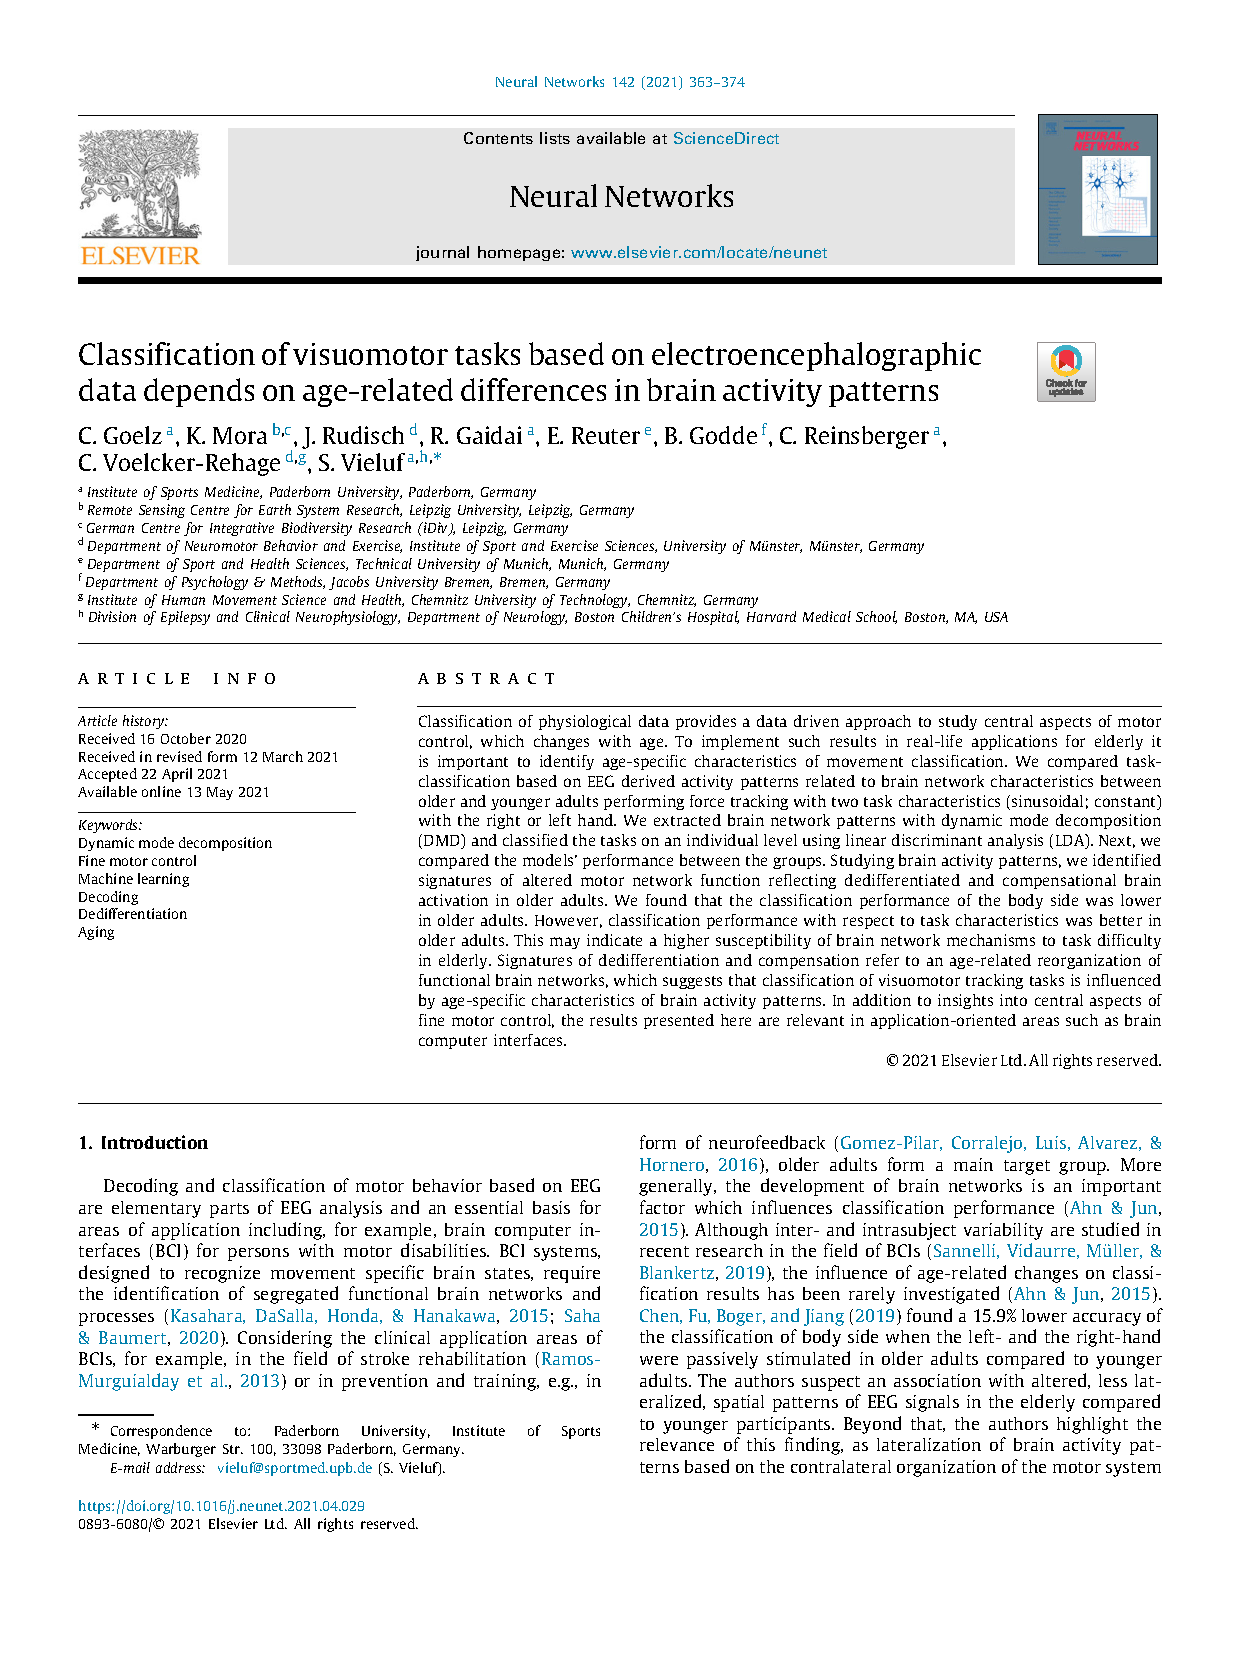
\includepdf[pages=-]{published_paper/ForceControl.pdf}
    \section*{\vspace*{\fill}\centering{Published Research Article \uproman{2}}\vspace*{\fill}}
        \addcontentsline{toc}{section}{Published Research Article \uproman{2}}
        \label{pub:paperII}
        % 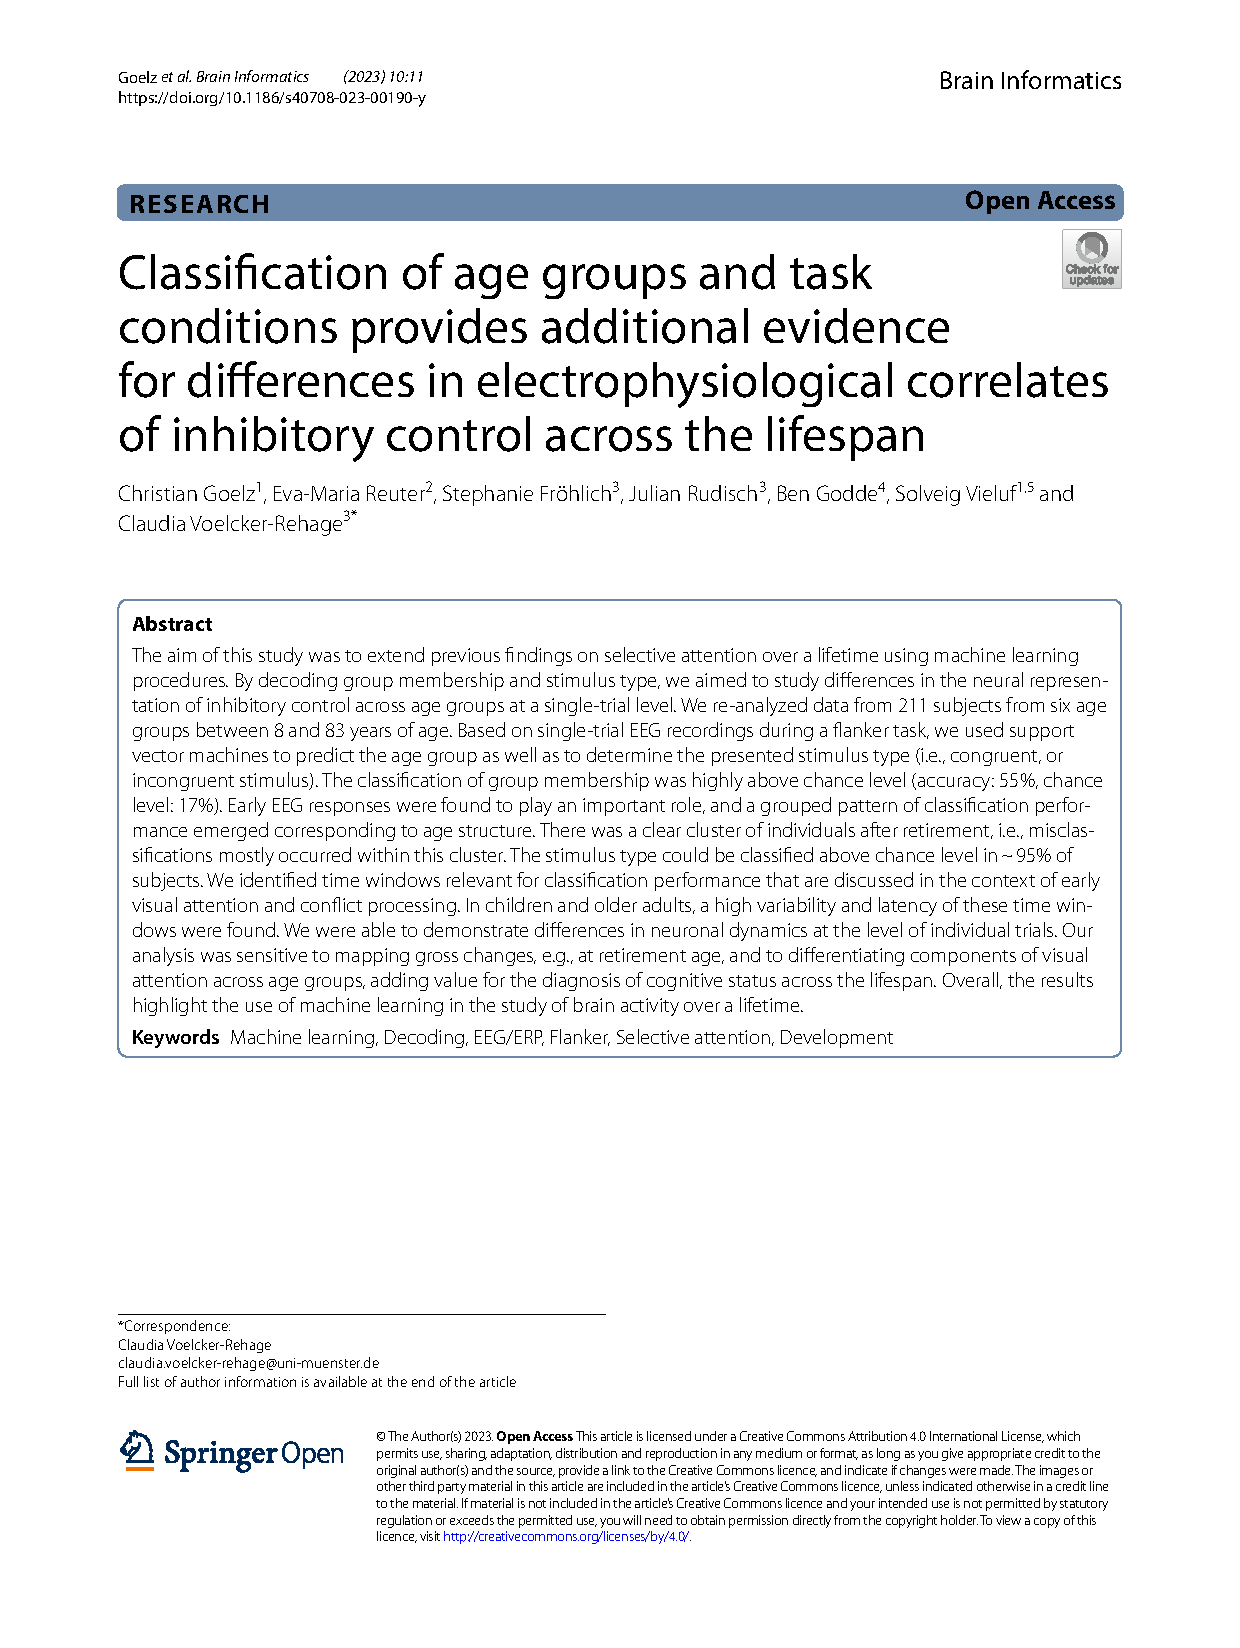
\includepdf[pages=-]{published_paper/Attention.pdf}
    \section*{\vspace*{\fill}\centering{Published Research Article \uproman{3}}\vspace*{\fill}}
        \addcontentsline{toc}{section}{Published Research Article \uproman{3}}
        \label{pub:paperIII}
        % 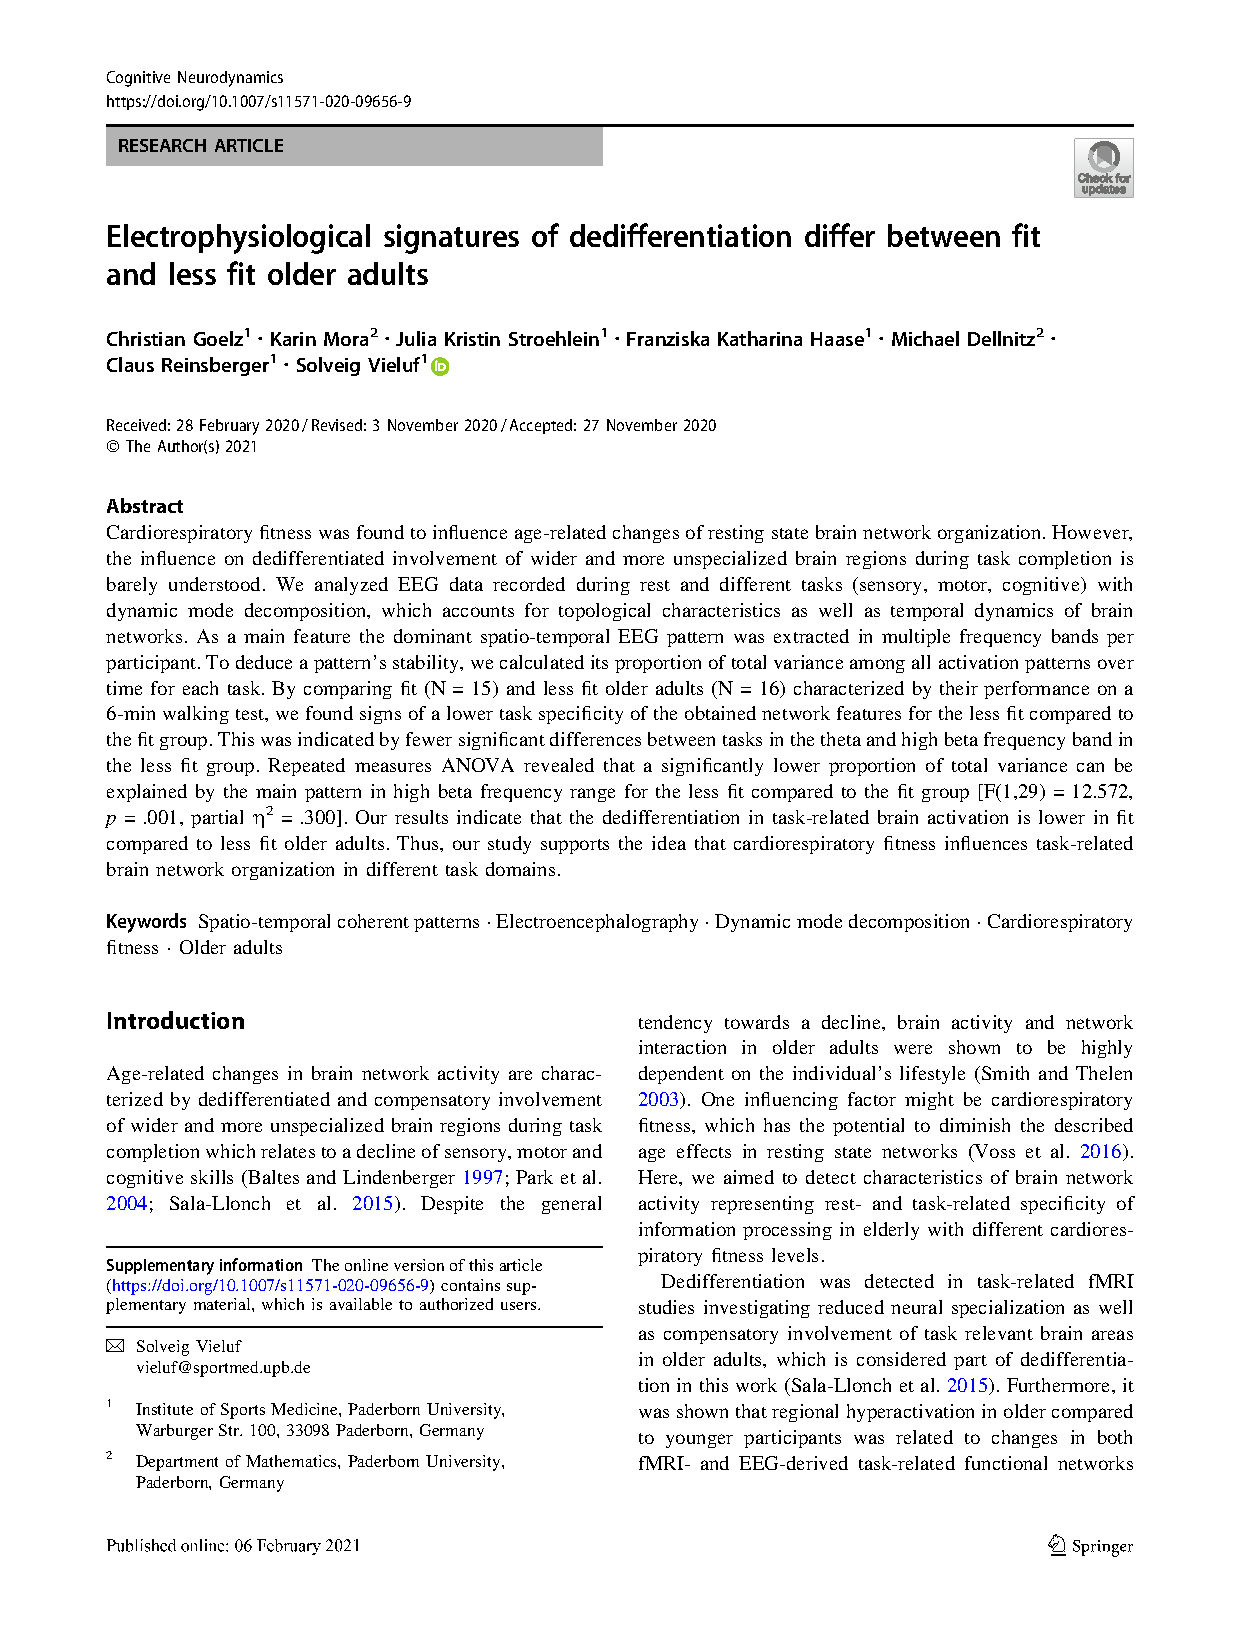
\includepdf[pages=-]{published_paper/Fitness.pdf}
    \section*{\vspace*{\fill}\centering{Published Research Article \uproman{4}}\vspace*{\fill}}
        \addcontentsline{toc}{section}{Published Research Article \uproman{4}}
        \label{pub:paperIV}
        % 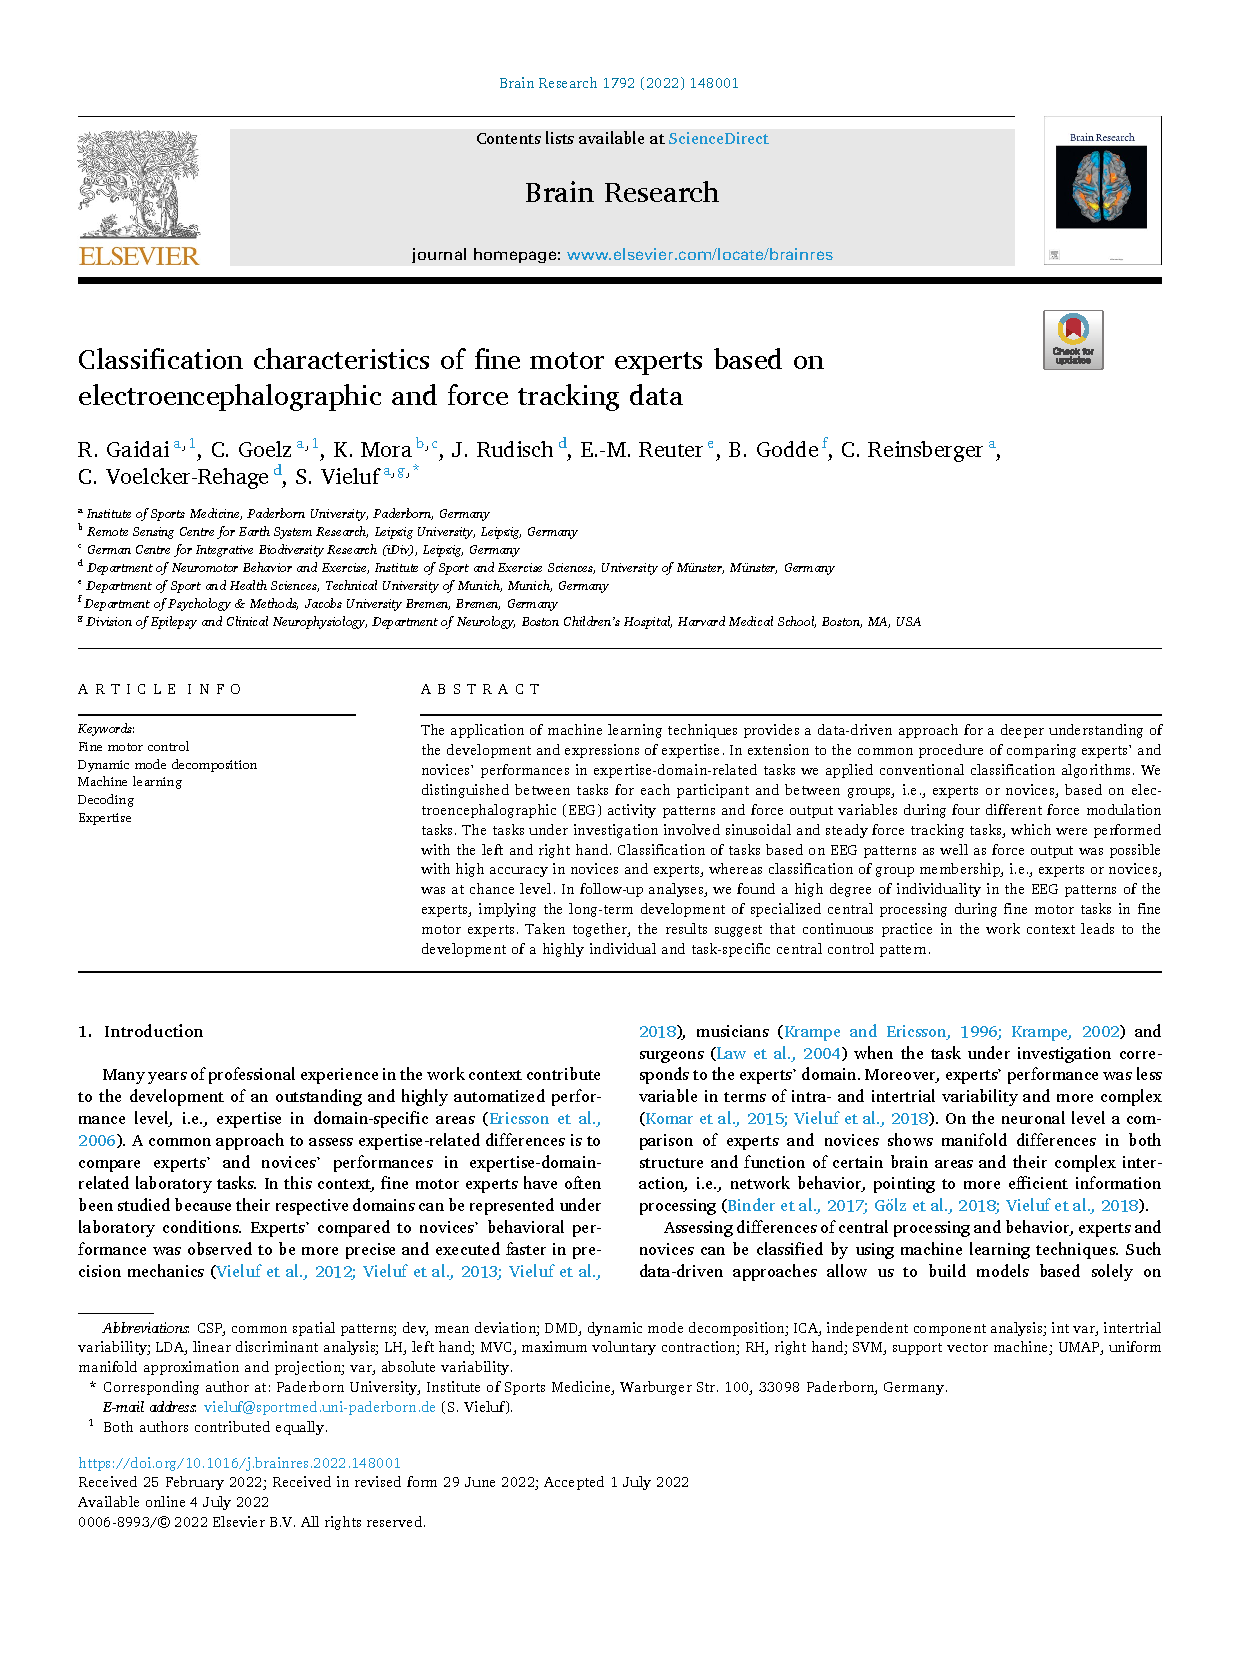
\includepdf[pages=-]{published_paper/Expertise.pdf}
\end{document}